\PassOptionsToPackage{notes}{handout}
\documentclass[main]{subfiles}
\setcounterrefbeforedot{chapter}{m-ws3-1}
\setcounterrefafterdot{section}{m-ws3-1}
\addtocounter{section}{-1}
\usepackage{solutions}

\begin{document}

\ifSubfilesClassLoaded{%
  \chaptermark{\chapterthree}
}{}

\section{Derivatives of Trig Functions} \label{ws3-1}

\probonly{
\begin{framed}
\textbf{Key Ideas}:
\begin{itemize}[topsep=0pt,partopsep=0pt,parsep=8pt,itemsep=0pt]

\item You should understand how we found $\frac{d}{dx} (\sin x)$ (although
  you don't need to be able to reproduce this argument on your own), and
  you should appreciate the importance of the two limits $\lim\limits_{x
    \to 0} \tfrac{\sin x}{x} = 1$ and $\lim\limits_{x \to 0} \tfrac{\cos x
    -1}{x} = 0$.

\item You should understand that the two limits $\lim\limits_{x \to 0}
  \tfrac{\sin x}{x} = 1$ and $\lim\limits_{x \to 0} \tfrac{\cos x -1}{x} =
  0$ are really just statements about the derivatives of $\sin x$ and
  $\cos x$ at $x = 0$.

\item You should know the derivatives of the six trigonometric functions
  $\sin x$, $\cos x$, $\tan x$, $\csc x$, $\sec x$, $\cot x$.

\item You should be able to use these new derivatives with techniques you
  already know, such as the Chain Rule and implicit differentiation.

\end{itemize}
\end{framed}
}

\begin{enumerate}
\item 
  \note{After sketching, students will probably immediately want to say
    that $\frac{d}{dx} (\sin x) = \cos x$, but I want them to realize that
    we don't know how ``tall'' the graph of $\frac{d}{dx} (\sin x)$ is
    since we don't know how steep the graph of $\sin x$ is at $x = 0$.
    So, more investigation is needed.}

  \begin{problem}[\stretch{2}]
    Sketch the graph of $\sin x$.  Based on this, sketch the graph of the
    derivative of $\sin x$.  From your graph, do you have a guess as to
    what the derivative of $\sin x$ might be?
  \end{problem}

  \begin{solution}
    Here's the graph of $\sin x$ (which should be totally familiar by
    now!): 
    \begin{center}
      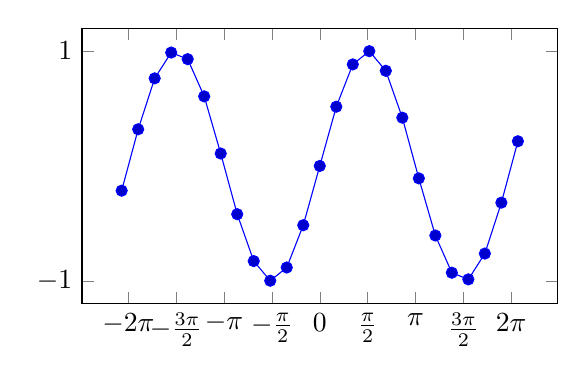
\begin{tikzpicture}
        \begin{axis}[xtick={-6.28, -4.71, ..., 6.28}, xticklabels={$-2
            \pi$, $-\frac{3\pi}{2}$, $-\pi$, $-\frac{\pi}{2}$, 0,
            $\frac{\pi}{2}$, $\pi$, $\frac{3\pi}{2}$, $2\pi$},
          ytick={-1, 1}, width=3in, height=2in]
          \addplot+[domain=-6.5:6.5]{sin(deg(x))};
        \end{axis}
      \end{tikzpicture}      
    \end{center}
    At $x = 0$, the slope is positive, and the slope decreases until it is
    0 at $\frac{\pi}{2}$.  It then continues decreasing until $\pi$, where
    it seems to be at its most negative.  It then becomes less negative,
    until $x = \frac{3 \pi}{2}$, where it's 0, and then it continues
    increasing.  That gives us the following graph of $\frac{d}{dx} (\sin
    x)$:
    \begin{center}
      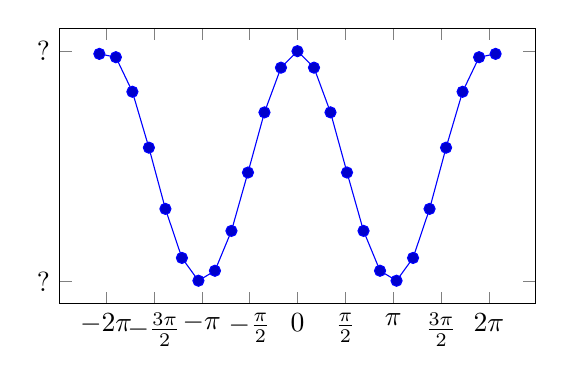
\begin{tikzpicture}
        \begin{axis}[xtick={-6.28, -4.71, ..., 6.28}, xticklabels={$-2
            \pi$, $-\frac{3\pi}{2}$, $-\pi$, $-\frac{\pi}{2}$, 0,
            $\frac{\pi}{2}$, $\pi$, $\frac{3\pi}{2}$, $2\pi$},
          ytick={-1, 1}, width=3in, yticklabels={?, ?}, height=2in]
          \addplot+[domain=-6.5:6.5]{cos(deg(x))};
        \end{axis}
      \end{tikzpicture}      
    \end{center}
    This graph should remind you of the graph of $\cos x$, but we don't
    have enough information from just the graph to be sure whether this is
    true.  For example, we don't know how steep the graph of $\sin x$ is
    at $x = 0$, so we don't know how high the graph of $\frac{d}{dx} (\sin
    x)$ should be at $x = 0$.  In addition, we can't tell just from the
    graph of $\sin x$ whether the oscillations of $\frac{d}{dx} (\sin x)$
    are actually sinusoidal or just close to being sinusoidal.
  \end{solution}

\item 
  \begin{enumerate}
  \item
    \begin{problem}[\vfill]
      What is the definition of the derivative of $\sin x$?
    \end{problem}

    \begin{solution}
      The derivative of $\sin x$ is $\boxed{\lim_{h \to 0}
        \frac{\sin(x+h) - \sin(x)}{h}}$. 
    \end{solution}

  \item
    \begin{problem}[\vfill]
      What is the definition of the derivative of $\sin x$ at $x = 0$?
    \end{problem}

    \begin{solution}
      The derivative of $\sin x$ at $x = 0$ is $\displaystyle \lim_{h \to
        0} \frac{\sin(0 + h) - \sin(0)}{h} = \boxed{\lim_{h \to 0}
        \frac{\sin(h)}{h}}$.
    \end{solution}

  \item
    \begin{problem}[\vfill]
      What is the definition of the derivative of $\cos x$ at $x = 0$?
    \end{problem}

    \begin{solution}
      This is $\displaystyle \lim_{h \to 0} \frac{\cos(0 + h) -
        \cos(0)}{h} = \boxed{\lim_{h \to 0} \frac{\cos(h) - 1}{h}}$.
    \end{solution}

  \item
    \begin{problem}[\vfill]
      Can you evaluate either of the derivatives in
      {{{{\#2}}(b)}} or
      {{{{\#2}}(c)}} just by thinking about the
      graphs of $\sin x$ and $\cos x$?
    \end{problem}

    \begin{solution}
      Just by thinking about the graph of $\cos x$, we can tell that the
      derivative of $\cos x$ at $x = 0$ is $0$; that tells us that the
      limit in {{{{\#2}}(c)}} is 0, so
      $\boxed{\lim_{h \to 0} \frac{\cos(h) - 1}{h} = 0}$.

      However, we can't tell the derivative of $\sin x$ at $x = 0$ just
      from the graph of $\sin x$. 
    \end{solution}

  \end{enumerate}

\pspace{\newpage}

\item 
  The limit $\displaystyle \lim_{h \to 0} \frac{\sin(h)}{h}$ is an
  interesting one. We will treat determining this limit as a separate problem for now and bring the result back into our original inquiry. Let's relabel $h$ as $A$ for the time being and consider $\displaystyle \lim_{A \to 0} \frac{\sin A}{A}$.

  \begin{enumerate}
  \item

    \note{In these first two parts, I simply want them to recognize that
      this limit can't be evaluated ``easily.''}

    \begin{problem}[0.25in]
      What is $\displaystyle \lim_{A \to 0} \sin A$?  Does that allow us
      to determine $\displaystyle \lim_{A \to 0} \frac{\sin A}{A}$ is?
    \end{problem}

    \begin{solution}
      $\displaystyle \lim_{A \to 0} \sin A = \sin(0) = 0$, but this does
      not automatically mean that $\displaystyle \lim_{A \to 0}
      \frac{\sin A}{A} = 0$.
    \end{solution}

  \item
    \begin{problem}[0.25in]
      What is $\displaystyle \lim_{A \to 0} A$?  Does that allow us to
      determine $\displaystyle \lim_{A \to 0} \frac{\sin A}{A}$ is?      
    \end{problem}

    \begin{solution}
      $\displaystyle \lim_{A \to 0} A = 0$, but this does not
      automatically mean that $\displaystyle \lim_{A \to 0} \frac{\sin A}{A} =
      \infty$ or $-\infty$.
    \end{solution}

  \end{enumerate}

  This limit is not so simple, so we'll have to use some ingenuity to find
  it.
  \begin{enumerate}[resume]

  \item
    \begin{problem}
      The following three pictures show a positive acute angle $A$
      on the unit circle in the first quadrant.  For each picture, find the length of the dotted segment or arc in terms of $A$.
    \end{problem}

      \NewDocumentCommand{\graphdiagram}
      {O{} O{} O{} m}{
        \coordinate (O) at (0,0);
        \coordinate (A) at (\rtheta{1}{#4});
        \coordinate (B) at (\rtheta{cos(#4)}{#4});
        \coordinate (C) at (\rtheta{cos(#4)}{0});
        \coordinate (D) at (1,0);
        
        \addplot[domain=#4:90, data cs=polar, thick] (x,1);
        
        \addplot[domain=0:#4, data cs=polar, #3] (x,1);
        \addplot[domain=0:#4, data cs=polar, #1] (x,{cos(#4)});
        \addplot[domain=0:{sin(#4)}, #2] ({cos(#4)},x);
            
        \draw[thick] (O) -- (A);
        \draw pic[draw=black, angle radius = 18, 
            angle eccentricity = 0.7, "$A$"]
            {angle=D--O--A};
        \filldraw[radius=2pt] (A) circle {} (B) circle {}
            (C) circle {} (D) circle;
            
      }
      \begin{center}
        \begin{tikzpicture}
        \begin{groupplot}[
        group style={group size=3 by 1},
        xmin=-0.15, xmax=1.15,
        ymin=-0.15, ymax=1.15,
        xtick={1},ytick={1},
        unit vector ratio*={1 1},
        width=2.5in
        ]
        \nextgroupplot
        \graphdiagram[][red, ultra thick,
        densely dashed][]{45}
        \solonly{
        \node[text=red,fill=white] at 
        ({cos(45)+0.17},{sin(45)/2})
            {$\sin A$};
            }

        \nextgroupplot
        \graphdiagram[][][orange, ultra thick,
        densely dashed]{45}
        \solonly{
            \node[text=orange] at 
            (\rtheta{1.1}{22.5}) {$A$};
            }

        \nextgroupplot
        \graphdiagram[blue, ultra thick,
        densely dashed][][]{45}
        \solonly{
            \node[text=blue] at 
            (\rtheta{0.7*cos(45)}{22.5})
            {$A\cos A$};
            }

        \end{groupplot}
        \end{tikzpicture}
      \end{center}

      \begin{solution}
      In the first picture, the length of the red
      segment is the $y$-coordinate of the point that $A$
      determines on the unit circle, so its length is $\sin A$.

      In the second picture, the orange arc has radius 1 and is subtended by $A$, so its length is $A$.

      In the third picture, the blue arc has radius $\cos A$ and is subtended by $A$, so its length is
      $A\cos A$.
      \end{solution}

      \pspace{0.5in}

  \item

    \note{Here, there is a Squeeze Theorem argument.  Students have not
      formally been introduced to the Squeeze Theorem, but they usually
      find the idea pretty intuitive.}

    Put the three lengths in increasing order:
    \[ \cfitb{1in}{{A \cos A}} 
    < \cfitb{1in}{{ \sin A}}
    < \cfitb{1in}{{ A}} \]
    Now divide by $A$ (which is positive because $A > 0$).
    \[ \cfitb[\vphantom{\frac{a}{b}}]{1in}{\cos A } 
    < \cfitb[\vphantom{\frac{a}{b}}]{1in}{\frac{\sin A}{A}} 
    < \cfitb[\vphantom{\frac{a}{b}}]{1in}{1}
    \]

    What happens as $A \to 0^+$?

    \begin{solution}
      As $A\to 0^+$, ${\cos A} \to 1$. So $\frac{\sin
        A}{A}$ gets ``squeezed'' between 1 and something that approaches
      1. Therefore, $\displaystyle \lim_{A\to 0^+}\frac{\sin A}{A} = 1$.
    \end{solution}

    \pspace{0.5in}

  \item

    \note{I'll use the fact that $\dfrac{\sin A}{A}$ is an even function
      of $A$ to explain why the left-hand limit is the same as the
      right-side limit.}

    \begin{problem}[0.5in]
      What does that tell you about $\displaystyle
      \lim_{A \to 0} \frac{\sin A}{A}$?
    \end{problem}

    \begin{solution}
      Since $\dfrac{\sin A}{A}$ is an even
      function, this also means that $\displaystyle \lim_{A \to 0^-}
      \frac{\sin A}{A} = 1$, so the two-sided limit $\displaystyle \lim_{A
        \to 0} \frac{\sin A}{A}$ is equal to $\boxed{1}$.
    \end{solution}

  \item
    \begin{problem}[0.5in]
      In this argument, it was important that $A$ was measured in
      radians.  Which step would be wrong if we measured $A$ in degrees? 
    \end{problem}

    \begin{solution}
      We used the fact that $A$ was measured in radians to
      find the lengths of the two arcs. If $A$ was in degrees,
      the arc length formula $s=rA$ would not valid.
    \end{solution}
  \end{enumerate}  

\end{enumerate}

\begin{framed}
    \begin{minipage}{0.46\textwidth}
    \textbf{Sandwich Theorem/Squeeze Theorem}
    \vspace{6pt}
    
    If $f(x) \leq j(x) \leq g(x)$ for all $x$ in the vicinity of $a$
    (although not necessarily at $a$), and
    \[\displaystyle\lim_{x\to a}f(x) = \lim_{x\to a} g(x) = L,\]
    then
    \[\displaystyle\lim_{x\to a}j(x) = L.\]
    \end{minipage}
    \hspace{20pt}
    \begin{minipage}{0.45\textwidth}
    \centering
    
\includegraphics{images/gottlieb-sandwich.pdf}
    
    $j$ is ``sandwiched/squeezed" between $f$ and $g$
    \end{minipage}
\end{framed}

\begin{enumerate}[resume]

\item 
  There's just one more fact we need to find the derivative of $\sin x$:

  \begin{framed}
    \textbf{Fact.} $\sin(A + B) = \sin A \cos B + \sin B \cos A$.  (You
    don't need to remember this formula, but you should definitely remember
    that $\sin(A + B) \neq \sin A + \sin B$!)
  \end{framed}

  We've already seen in {{{{\#2}}(a)}} that
  \begin{align*}
    \frac{d}{dx} (\sin x) &= \lim_{h \to 0}\frac{\sin (x +
      h) - \sin x}{h} \\
    \intertext{Use the fact that $\sin(A + B) = \sin A \cos B + \sin B
      \cos A$ to rewrite the previous line:} %
    &= \lim_{h \to 0} \fitb[\vphantom{\dfrac{a}{b}}]{3in}{\displaystyle
      \frac{\sin x \cos h + \sin h \cos x -
        \sin x}{h}} \\
    \intertext{Rearrange the previous line to group together the terms
      involving $\sin x$ and the terms involving $\cos x$, and then factor
      $\sin x$ and $\cos x$ out of their respective expressions:} %
    &= \lim_{h \to 0} \left[ \sin x \left(
        \fitb[\vphantom{\dfrac{a}{b}}]{1.5in}{\displaystyle \frac{\cos h -
            1}{h}} \right) + \cos x \left(
        \fitb[\vphantom{\dfrac{a}{b}}]{1.5in}{\displaystyle \frac{\sin
            h}{h}} \right) \right] \\
    \intertext{You should recognize the two expressions you just wrote and
      be able to find the limit of each as $h \to 0$:}%
    &= \fitb[\vphantom{\dfrac{a}{b}}]{2in}{(\sin x) \cdot 0 + (\cos x)
      \cdot 1 = \cos x} \solonly{\text{\textbf{ by
          {{{{\#2}}(d)}} and {{\#3}}}}}
  \end{align*}
  \begin{framed}
    \emph{\textbf{Note:} This is only true when $x$ is in radians.}
  \end{framed}


\item 
  \begin{problem}[\vfill]
    What is the derivative of $\cos x$?
  \end{problem}

  \begin{solution}
    It's easiest to use the fact that the graph of $\cos x$ is a
    horizontal shift of the graph of $\sin x$; if we shift the graph of
    $\sin x$ left by $\frac{\pi}{2}$, we get the graph of $\cos x$.  That
    is, $\cos (x) = \sin \left( x + \frac{\pi}{2} \right)$.  Therefore,
    \begin{align*}
      \frac{d}{dx} (\cos x) &= \frac{d}{dx} \left[ \sin \left( x +
          \frac{\pi}{2} \right) \right] \\
      &= \cos \left( x + \frac{\pi}{2} \right) \cdot 1 \text{ by the Chain
        Rule} 
    \end{align*}
    The graph of $\cos \left( x + \frac{\pi}{2} \right)$ is the graph of
    $\cos x$ shifted left by $\frac{\pi}{2}$, which is the same as
    $\boxed{-\sin x}$. 
  \end{solution}

\item 

  \begin{problem}[\vfill\newpage]
    Find the derivative of $\tan x$.  \emph{Do} simplify your answer.
  \end{problem} 

  \begin{solution}
    We can use the Quotient Rule on $\displaystyle \tan x = \frac{\sin
      x}{\cos x}$ (or, equivalently, use the Product Rule and Chain Rule
    on $(\sin x) (\cos x)^{-1}$) to get:
    \begin{align*}
      \frac{d}{dx} (\tan x) &= \frac{(\cos x)(\cos x) - (\sin x) (-\sin
        x)}{(\cos x)^2} \\
      &= \frac{\cos^2 x + \sin^2 x}{\cos^2 x} \\
      &= \frac{1}{\cos^2 x} \\
      &= \sec^2 x
    \end{align*}
  \end{solution}

\end{enumerate}
%\begin{problemonly}
  \begin{framed}
    \textbf{Derivatives of the six basic trigonometric functions.}  (You
    should memorize these.)

    \begin{multicols}{3}
    
      $\dfrac{d}{dx} (\sin x) = \fitb{1in}{\cos x}$

      $\dfrac{d}{dx} (\csc x) = - \csc x \cot x$

      $\dfrac{d}{dx} (\cos x) = \fitb{1in}{-\sin x}$

      $\dfrac{d}{dx} (\sec x) = \sec x \tan x$

      $\dfrac{d}{dx} (\tan x) = \fitb{1in}{\sec{^2} x}$

      $\dfrac{d}{dx} (\cot x) = -\csc^2 x$
      
    \end{multicols}
    \vspace{-8pt}
    (You'll show the last three on your homework.)
  \end{framed}
%\end{problemonly}


\begin{enumerate}[resume]
\item 
 Find derivatives of the
  following functions.  (Don't worry about simplifying your answers.)
  Which differentiation rules do you need in each part? 

  \begin{enumerate}
  \item
    \begin{problem}[\vfill]
      $f(x) = \pi \cos(12 x)$
    \end{problem}

    \begin{solution}
      By the Chain Rule, $f'(x) = \pi [ -\sin(12 x) \cdot 12] = \boxed{-12
        \pi \sin (12x)}$.
    \end{solution}

  \item
    \begin{problem}[\vfill\vfill]
      $f(x) = x \sin \left( x^3 \right)$, $g(x) = x \sin^3 x$, and $h(x) =
      x (\sin x)^3$.  (Are these the same or different?)
    \end{problem}

    \begin{solution}
      First, $h(x)$ is the same as $g(x)$.  To differentiate $f(x)$ and
      $g(x)$, we start with the Product Rule: 
      \begin{align*}
        f'(x) &= x \cdot \frac{d}{dx} \left[ \sin \left( x^3 \right)
        \right] + \sin \left( x^3 \right) \\
        &= \boxed{x \cdot \cos \left(x^3 \right) \cdot 3x^2 + \sin
          \left( x^3 \right)}
      \end{align*}
      and
      \begin{align*}
        g'(x) = h'(x) &= x \cdot \frac{d}{dx} \left[ (\sin x)^3 \right] +
        (\sin x)^3
        \text{ by the Product Rule} \\
         &= \boxed{x \cdot 3 (\sin x)^2 \cos x + (\sin x)^3}
      \end{align*}      
    \end{solution}

  \item
    \begin{problem}[\vfill\newpage]
      $f(x) = 6 \cos (\ln x)$
    \end{problem}

    \begin{solution}
      Using the Chain Rule, $\boxed{f'(x) = -6\sin(\ln x)\cdot x^{-1}}$.
    \end{solution}

  \item

    \note{Students sometimes get confused when using the Chain Rule with
      $\sec$ because the derivative of $\sec$ is already a product.}

    \begin{problem}[\vfill\vfill]
      $f(x) = \pi \sec ( x^2 - x)$, $g(x) = \pi \sec \left( x^2 \right) -
      x$ (How are these functions different?)
    \end{problem}

    \begin{solution}
      To differentiate $f$, we need to use the Chain Rule with  inner
      function $x^2-x$:
      \[ \boxed{f'(x) = \pi \cdot \sec(x^2-x)\tan(x^2-x) \cdot (2x -
        1)}.\] To differentiate $g(x)$, we need to use the Chain Rule with
      inner function $x^2$:
      \[ \boxed{g'(x) = \pi \cdot \sec(x^2)\tan(x^2) \cdot 2x - 1}.\] Note
      that we \textbf{need} parentheses around $2x-1$ in $f'(x)$ and that
      we should \textbf{not} have parentheses around $2x-1$ for $g'(x)$.
    \end{solution}

  \item
    \begin{problem}[\vfill]
      $f(x) = \sin^2 x \cos^2 x$
    \end{problem}

    \begin{solution}
      First, we need the Product Rule:
      \begin{align*}
        f'(x) = {} & \frac{d}{dx}
        \left(\fcolorbox{green}{white}{$\displaystyle \cos^2 x $}\cdot
          \fcolorbox{green}{white}{$\displaystyle  \sin^2 x $}\right) \\
        = {} & \cos^2 x \cdot \frac{d}{dx}
        \left(\fcolorbox{red}{white}{$\displaystyle
            \fcolorbox{blue}{white}{$\displaystyle \sin x$}^ { 2}
            $}\right)+ \frac{d}{dx}
        \left(\fcolorbox{red}{white}{$\displaystyle
            \fcolorbox{blue}{white}{$\displaystyle \cos x$}^ { 2}
            $}\right)\cdot \sin^2 x \\
        \intertext{And now we use the Chain Rule:} %
        = {} & \boxed{\cos^2 x \cdot \left(2 \sin x \cdot \cos x\right)+
          \left(2 \cos x \cdot -\sin x\right)\cdot \sin^2 x}
      \end{align*}
    \end{solution}

  \item
    \begin{problem}[\vfill\newpage]
      $f(x) = \sin^2\!\left( x^2 \right) + \cos^2\!\left( x^2 \right)$
    \end{problem}

    \begin{solution}
      By the Pythagorean Identity, the formula for $f$ simplifies to $f(x)
      = 1$, so $f'(x) = \boxed{0}$. 
    \end{solution}

  \end{enumerate}

\item 
  For each of the functions below, your job is to sketch the graph
  on the interval $[0,4\pi]$.
  \begin{enumerate}[topsep=0pt]
  \item

    \begin{problem}
      Graph $f(x)=\sin x + x$.

      Before you get started, try to imagine what the graph could look
      like. What do you wonder about? (You do not need to write this part down.
    \end{problem}

      \begin{enumerate}[topsep=0pt]
        \item
        \begin{problem}
          Identify all critical points on $[0,4\pi]$.
          Classify them as max/min or point of inflection.
        \end{problem}

        \begin{solution}
           To find the 
            critical points, we need to analyze $f'(x)=\cos x +1$. $f'(x)$
            is never undefined. We set $f'(x)=0$ and solve for $x$:
            \vspace{-6pt}
            \begin{align*}
                \cos x + 1 &= 0 \\
                \cos x &= -1 \\
                x &= \pi,\,3\pi
            \end{align*}
            The critical points are \fbox{$\pi$, $3\pi$.} We can
            observe that $f'(x)=\cos x +1$ is always non-negative, since the
            balance value is 1 and the amplitude is 1. This means that $f$
            is always increasing, so we have inflection points at $x=\pi$,
            $3\pi$. We can visualize this with the following
            sign chart:
            \begin{center}
            \begin{tikzpicture}
            \begin{axis}[xmin=-5, xmax=4*pi,
              ymin = -1, ymax=4.5, axis y line=none, 
              x axis line style={-},
              xtick={0,pi,3*pi,4*pi}, 
              xticklabels={$0$,$\pi$,$3\pi$,$4\pi$},
              height=2in,width=4in,clip=false]
              \draw (-5,0.5) node[right] {$f$};
              \draw (-5,-0.5) node[right] {sign of $f'$};
              \draw (pi/2,-0.5) node {$+$};
              \draw (2*pi,-0.5) node {$+$};
              \draw (7*pi/2,-0.5) node {$+$};
              \draw[->] (0,0.5) -- (pi-0.5,1.5);
              \draw[->] (pi-0.5,1.5) -- (pi+0.5,1.5);
              \draw[->] (pi+0.5,1.5) -- (3*pi-0.5,3);
              \draw[->] (3*pi-0.5,3) -- (3*pi+0.5,3);
              \draw[->] (3*pi+0.5,3) -- (4*pi,4.5);
            \end{axis}
            \end{tikzpicture}
            \end{center}
            
        \end{solution}

        \item
        \begin{problem}
          Is this function periodic? Why or why not?
        \end{problem}

        \begin{solution}
            The function cannot be periodic, because it is continuous and
            always increasing, so the graph will never repeat.
        \end{solution}
        
        \item 
        \begin{problem}[\vfill]
          Sketch the graph of $y=\sin x +x$ on the interval $[0,4\pi]$.     
        \end{problem}

        \begin{solution}
        We can start by plotting a few points, e.g. $(0,0)$, $(\pi,\pi)$, $(3\pi,3\pi)$, and $(4\pi, 4\pi)$. We know that
        there are inflection points at $x=\pi$ and $3\pi$, and the function
        is always increasing.
            \begin{center}
            \begin{tikzpicture}
            \begin{axis}[xmin=0, xmax=4*pi+0.5,
              ymin = 0, ymax = 4*pi+0.5,
              xtick={pi,2*pi,3*pi,4*pi}, xticklabels={$\pi$,$2\pi$,
              $3\pi$,$4\pi$},ytick={pi,2*pi,3*pi,4*pi}, yticklabels={$\pi$,
              $2\pi$,$3\pi$,$4\pi$}]
              \addplot[domain=0:4*pi]{sin(deg(x))+x};
            \end{axis}
            \end{tikzpicture}
            \end{center}
        \end{solution}
      \end{enumerate}


  \item
    \begin{problem}[\vfill]
        Graph $g(x)=2\sin x + x$. Follow the same directions as parts (a)i--(a)iii.
    \end{problem}
    
    \begin{solution}
        To find the
        critical points, we need to analyze $g'(x)=2\cos x +1$. $g'(x)$
        is never undefined. Setting $g'(x)=0$ and solving for $x$:
        \vspace{-6pt}
        \begin{align*}
            2 \cos x + 1 &= 0 \\
            \cos x &= -\tfrac{1}{2} \\
            x &= \tfrac{2\pi}{3},\tfrac{4\pi}{3},\tfrac{8\pi}{4},\tfrac{10\pi}{3}
        \end{align*}
        The critical points are $\frac{2\pi}{3}$, $\frac{4\pi}{3}$,
        $\frac{8\pi}{4}$, and
        $\frac{10\pi}{3}$. To classify them,
        we can draw a sign chart for $g'$. By envisioning the graph of $g'(x)=
        2\cos x +1$, we can deduce that $g'(x)$ is positive at $x=0$, and it
        changes sign at each $x$-intercept.
        \begin{center}
        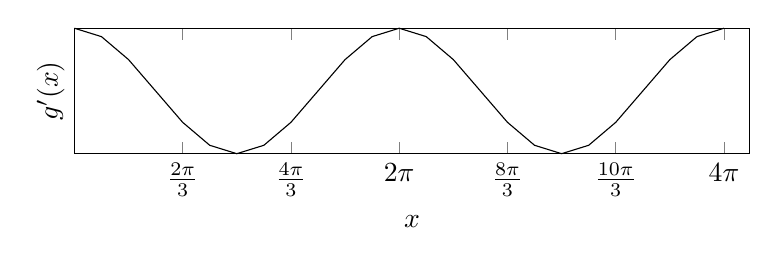
\begin{tikzpicture}
        \begin{axis}[xmin=0, xmax=4*pi+0.5, ymin = -1, ymax = 3,
              xlabel=$x$, ylabel=$g'(x)$,
              xtick={2*pi/3,4*pi/3,2*pi,8*pi/3,10*pi/3,4*pi},
              xticklabels={$\frac{2\pi}{3}$,$\frac{4\pi}{3}$,
              $2\pi$,$\frac{8\pi}{3}$,$\frac{10\pi}{3}$,$4\pi$},
              ytick=\empty, height=1.25in, width=4in, clip=false]
              \addplot[domain=0:4*pi]{2*cos(deg(x))+1};
        \end{axis}
        \end{tikzpicture}
        \end{center}
        
        \begin{center}
        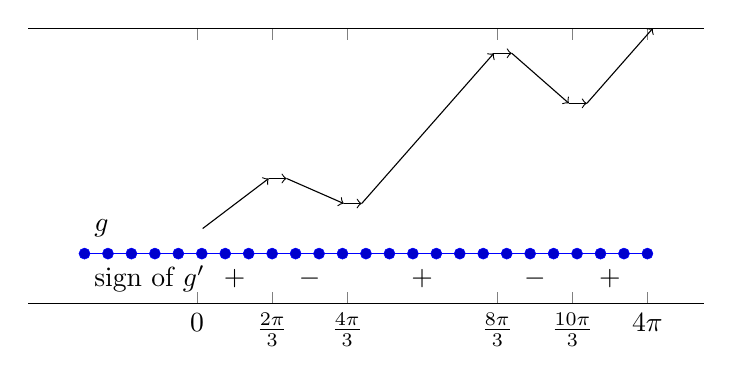
\begin{tikzpicture}
          \begin{axis}[axis y line=none, x axis line style={-}, xtick={0, 2*pi/3,
          4*pi/3,8*pi/3,10*pi/3,4*pi}, xticklabels={$0$, $\frac{2\pi}{3}$,
          $\frac{4\pi}{3}$, $\frac{8\pi }{3}$, $\frac{10\pi}{3}$, $4\pi$}, ymin=-1, ymax=4.5, height=2in, width=4in, clip=false]
            \addplot+[domain=-pi:4*pi, very thin]{0};
            \draw (axis cs: -pi, -0.5) node[right] {sign of $g'$};
            \draw (axis cs: -pi, 0.5) node[right] {$g$};
            \draw (axis cs: pi/3, -0.5) node{$+$};
            \draw (axis cs: pi, -0.5) node{$-$};
            \draw (axis cs: 2*pi, -0.5) node{$+$};
            \draw (axis cs: 3*pi, -0.5) node{$-$};
            \draw (axis cs: 11*pi/3, -0.5) node{$+$};
            
            \draw[->, xshift=2pt] (axis cs: 0, 0.5) -- 
              (axis cs: 2*pi/3-0.25, 1.5);
            \draw[->, xshift=2pt] (axis cs: 2*pi/3-0.25, 1.5) -- 
              (axis cs: 2*pi/3+0.25, 1.5);
            \draw[->, xshift=2pt] (axis cs: 2*pi/3+0.25, 1.5) -- 
              (axis cs: 4*pi/3-0.25, 1);
            \draw[->, xshift=2pt] (axis cs: 4*pi/3-0.25, 1) -- 
              (axis cs: 4*pi/3+0.25, 1);
            \draw[->, xshift=2pt] (axis cs: 4*pi/3+0.25, 1) --
              (axis cs: 8*pi/3-0.25, 4);
            \draw[->, xshift=2pt] (axis cs: 8*pi/3-0.25, 4) -- 
              (axis cs: 8*pi/3+0.25, 4);
            \draw[->, xshift=2pt] (axis cs: 8*pi/3+0.25, 4) --
              (axis cs: 10*pi/3-0.25, 3);
            \draw[->, xshift=2pt] (axis cs: 10*pi/3-0.25, 3) -- 
              (axis cs: 10*pi/3+0.25, 3);
            \draw[->, xshift=2pt] (axis cs: 10*pi/3+0.25, 3) --
              (axis cs: 4*pi, 4.5);
            
          \end{axis}
        \end{tikzpicture}
        \end{center}
        Thus, $g$ has \fbox{local minima at $\frac{4\pi}{3}$, and
        $\frac{10\pi}{3}$,} and \fbox{local maxima at $x=\frac{2\pi}{3}$,
        $\frac{8\pi}{3}$.}

        The function is not periodic. $2\sin x$ has a period of $2\pi$, but $x$
        is not periodic, which means $g(x)$ cannot be periodic.

        To sketch the graph of $y=2\sin x+x$, we can start by plotting the
        relative extrema and endpoints, which are $(0,0)$, $(\frac{2\pi}{3},
        \frac{2\pi}{3}+\sqrt{3})$, $(\frac{4\pi}{3},\frac{4\pi}{3}-\sqrt{3})$,
         $(\frac{8\pi}{3},\frac{8\pi}{3}+\sqrt{3})$, $(\frac{10\pi}{3},
         \frac{10\pi}{3}-\sqrt{3})$, and $(4\pi,4\pi)$. We can use the sign
         chart to determine where $g$ is increasing and decreasing.
            \begin{center}
            \begin{tikzpicture}
            \begin{axis}[xmin=0, xmax=4*pi+0.5, ymin = 0, ymax = 4*pi+0.5,
              xlabel=$x$, ylabel=$g(x)$, 
              xtick={2*pi/3,4*pi/3,2*pi,8*pi/3,10*pi/3,4*pi},
              xticklabels={$\frac{2\pi}{3}$,$\frac{4\pi}{3}$,
              $2\pi$,$\frac{8\pi}{3}$,$\frac{10\pi}{3}$,$4\pi$},
              ytick={2*pi/3,4*pi/3,2*pi,8*pi/3,10*pi/3,4*pi},
              yticklabels={$\frac{2\pi}{3}$,$\frac{4\pi}{3}$,
              $2\pi$,$\frac{8\pi}{3}$,$\frac{10\pi}{3}$,$4\pi$}]
              \addplot[domain=0:4*pi]{2*sin(deg(x))+x};
            \end{axis}
            \end{tikzpicture}
            \end{center}
         
        
    \end{solution}
  \end{enumerate}

\end{enumerate}

\end{document}